\documentclass[12pt]{article}

\usepackage[english]{babel}
\usepackage[utf8]{inputenc}
\usepackage[top=2cm, left=2cm, right=2cm, bottom=2cm]{geometry}
\usepackage[document]{ragged2e}
\usepackage{tikz,minted,times}

\setlength\parindent{0pt}
\sloppy
\usetikzlibrary{automata,positioning,arrows,fit}
\tikzset{node distance=2.5cm,every state/.style={semithick,fill=gray!10},initial text={},double distance=2pt,every edge/.style={draw,->,>=stealth,auto,semithick}}
\usemintedstyle{colorful}

\title{COMP SCI 7411 Event Driven Computing Practice 3 Plan}
\author{Tinson Lai \\ a1812422}
\date{}

\begin{document}

\maketitle

Due to the constraint that train will not change direction, the following routes are the only options for trains entering the system.

\begin{itemize}
  \item Train entering from $1$ going east

    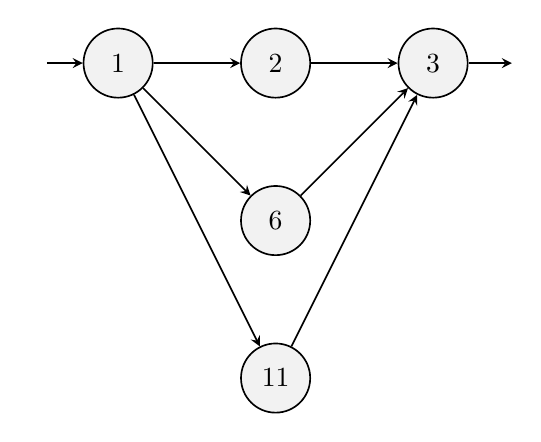
\begin{tikzpicture}
      \node[state, initial] at (0, 4) (1){1};
      \node[state] at (2, 4) (2){2};
      \node[state] at (2, 2) (6){6};
      \node[state] at (2, 0) (11){11};
      \node[state] at (4, 4) (3){3};

      \draw

      (1) edge (2)
      (1) edge (6)
      (1) edge (11)

      (2) edge (3)
      (6) edge (3)
      (11) edge (3)

      (3) edge +(1, 0)

      ;
    \end{tikzpicture}
  \item Train entering from $4$ going east

    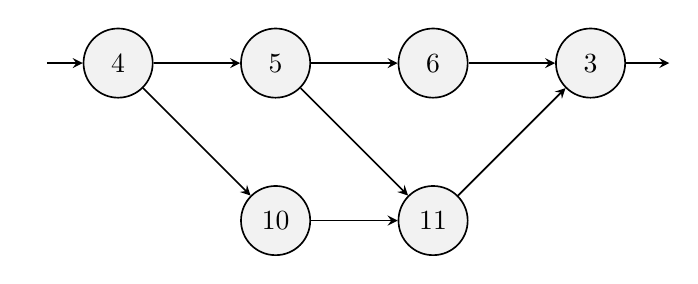
\begin{tikzpicture}
      \node[state, initial] at (0, 2) (4){4};
      \node[state] at (2, 2) (5){5};
      \node[state] at (4, 2) (6){6};
      \node[state] at (6, 2) (3){3};
      \node[state] at (2, 0) (10){10};
      \node[state] at (4, 0) (11){11};

      \draw

      (4) edge (5)
      (4) edge (10)

      (5) edge (6)
      (5) edge (11)
      (10) edge (11)

      (6) edge (3)
      (11) edge (3)

      (3) edge +(1, 0)

      ;
    \end{tikzpicture}
  \item Train entering from $8$ going west

    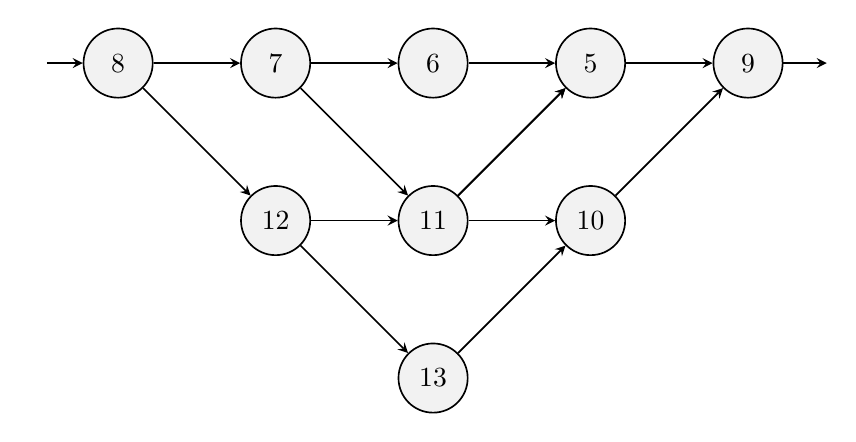
\begin{tikzpicture}
      \node[state, initial] at (0, 4) (8){8};
      \node[state] at (2, 4) (7){7};
      \node[state] at (4, 4) (6){6};
      \node[state] at (6, 4) (5){5};
      \node[state] at (8, 4) (9){9};
      \node[state] at (2, 2) (12){12};
      \node[state] at (4, 2) (11){11};
      \node[state] at (6, 2) (10){10};
      \node[state] at (4, 0) (13){13};

      \draw

      (8) edge (7)
      (8) edge (12)

      (7) edge (6)
      (7) edge (11)

      (12) edge (11)
      (12) edge (13)

      (11) edge (5)
      (11) edge (10)

      (13) edge (10)

      (6) edge (5)
      (11) edge (5)

      (5) edge (9)
      (10) edge (9)

      (9) edge +(1, 0)

      ;
    \end{tikzpicture}
\end{itemize}

Listing these routes is the first step to prevent potential deadlock due to those constraints. For example, a train driving east will never entre track $8$ which is actually the entrance for those trains driving west.

In the following sections, I will use the following notations in the Petri Net, where in the Petri Net tuple $N=\left(P,T,A,W,I\right)$

\begin{itemize}
  \item ($P$) $p_i$ refers to track $i$ when it's empty. $p_{i,e}$ or $p_{i,w}$ refers to track $i$ with a east direction ($e$) or west direction ($w$) train on it. This is a necessary notation to avoid deadlock.  All $p_i$ with $p_{i,e}$ and $p_{i,w}$ forms different buffers in the Petri Net.
  \item ($P$) $d_i$ refers to a dispatcher, where only $d_1$, $d_4$ and $d_8$ are available as trains can only enter the system from these tracks. They also act as producers in the Petri Net as well.
  \item ($P$) $o_i$ refers to the outgoing track, where only $o_3$ and $o_9$ are available as trains can only exit the system from these tracks. They also act as consumers in the Petri Net as well.
  \item ($T$) ${add_i}$ and ${out_i}$ means adding/removing a train from the inbound/outbound track.
  \item ($T$) $m_{i,j}$ refers to a move from track $i$ to track $j$ in train's own direction.
  \item ($T$) $m_{i,j}\left({p_{cond}}\right)$ means a movement is based on a condition of a track, where $p_{cond}$ should also be a state in the Petri Net. It is used to distinguished transition based on a precondition to avoid deadlock in the Petri Net.
  \item $W$ will always be one for all transitions. ($1$-safe)
  \item ($I$) All $p_i$, $d_i$ and $o_i$ will be an initial states as implied by the definition of producer, consumer and buffer. It is also obvious that the initial system will be completely empty, so the initial state should be neither $p_{i,e}$ nor $p_{1,w}$ but $p_i$.
\end{itemize}

\section{Tracks}

As the complete graph will still be very complex and difficult to draw, I will instead draw Petri Net for each track.

\subsection{Simple Transitions}

There are a few simple track which can be drawn without further consideration to avoid deadlock.

\subsubsection{Entrance}

The Petri Net for track $1$ will be

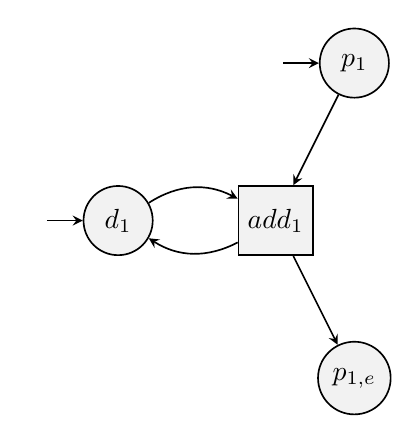
\begin{tikzpicture}
  \node[state, initial] at (0, 2) (d1){$d_1$};

  \node[state, initial] at (3, 4) (p1){$p_1$};
  \node[state] at (3, 0) (p1_e){$p_{1,e}$};

  \node[state, rectangle] at (2, 2) (add1){${add}_1$};

  \draw

  (d1) edge[bend left] (add1)
  (add1) edge[bend left] (d1)
  (p1) edge (add1)
  (add1) edge (p1_e)

  ;
\end{tikzpicture}

The Petri Net for track $4$ will be

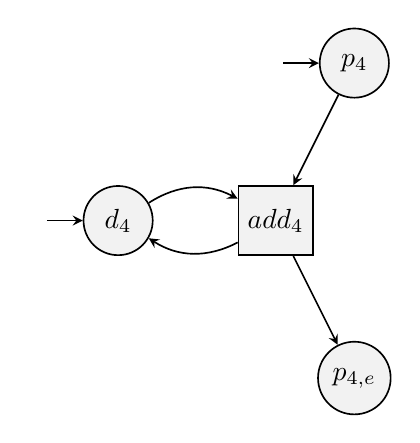
\begin{tikzpicture}
  \node[state, initial] at (0, 2) (d4){$d_4$};

  \node[state, initial] at (3, 4) (p4){$p_4$};
  \node[state] at (3, 0) (p4_e){$p_{4,e}$};

  \node[state, rectangle] at (2, 2) (add4){${add}_4$};

  \draw

  (d4) edge[bend left] (add4)
  (add4) edge[bend left] (d4)
  (p4) edge (add4)
  (add4) edge (p4_e)

  ;
\end{tikzpicture}

The Petri Net for track $8$ will be

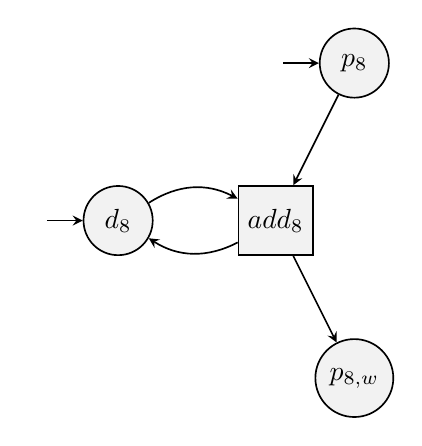
\begin{tikzpicture}
  \node[state, initial] at (0, 2) (d8){$d_8$};

  \node[state, initial] at (3, 4) (p8){$p_8$};
  \node[state] at (3, 0) (p8_w){$p_{8,w}$};

  \node[state, rectangle] at (2, 2) (add8){${add}_8$};

  \draw

  (d8) edge[bend left] (add8)
  (add8) edge[bend left] (d8)
  (p8) edge (add8)
  (add8) edge (p8_w)

  ;
\end{tikzpicture}

\subsubsection{Exit}

The graphs here will look a little bit weird as there is no outgoing arrow from the initial state. However, as said, this is only part of the complete graph.

The Petri Net for track $3$ will be

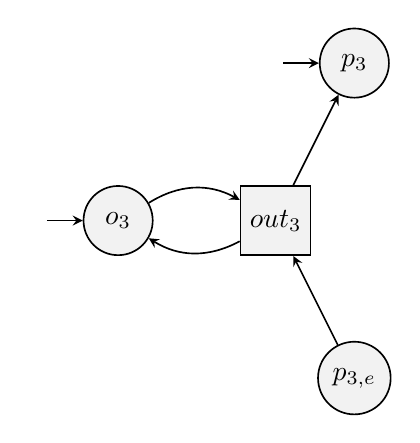
\begin{tikzpicture}
  \node[state, initial] at (0, 2) (o3){$o_3$};

  \node[state, initial] at (3, 4) (p3){$p_3$};
  \node[state] at (3, 0) (p3_e){$p_{3,e}$};

  \node[state, rectangle] at (2, 2) (out3){${out}_3$};

  \draw

  (p3_e) edge (out3)
  (out3) edge (p3)
  (o3) edge[bend left] (out3)
  (out3) edge[bend left] (o3)

  ;
\end{tikzpicture}

The Petri Net for track $9$ will be

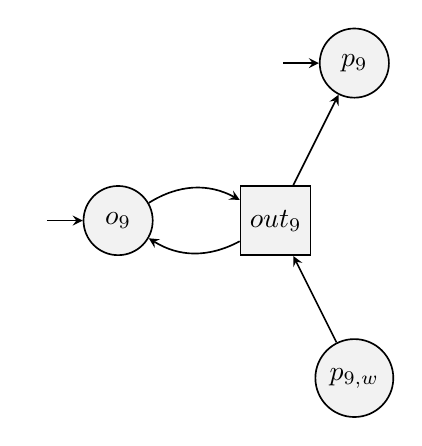
\begin{tikzpicture}
  \node[state, initial] at (0, 2) (o9){$o_9$};

  \node[state, initial] at (3, 4) (p9){$p_9$};
  \node[state] at (3, 0) (p9_w){$p_{9,w}$};

  \node[state, rectangle] at (2, 2) (out9){${out}_9$};

  \draw

  (p9_w) edge (out9)
  (out9) edge (p9)
  (o9) edge[bend left] (out9)
  (out9) edge[bend left] (o9)

  ;
\end{tikzpicture}

\subsubsection{Tracks with Simple Transition (East Direction)}

The following transitions involve two tracks and they will never entre a deadlock situation.

The Petri Net for $m_{1,2}$

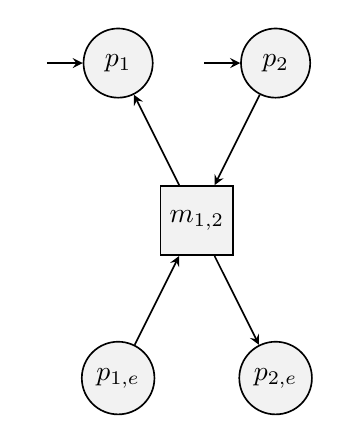
\begin{tikzpicture}
  \node[state, initial] at (3, 4) (p1){$p_1$};
  \node[state, initial] at (5, 4) (p2){$p_2$};

  \node[state] at (3, 0) (p1_e){$p_{1,e}$};
  \node[state] at (5, 0) (p2_e){$p_{2,e}$};

  \node[state, rectangle] at (4, 2) (m1_2){$m_{1,2}$};

  \draw

  (p1_e) edge (m1_2)
  (m1_2) edge (p1)
  (p2) edge (m1_2)
  (m1_2) edge (p2_e)

  ;
\end{tikzpicture}

The Petri Net for $m_{1,6}$

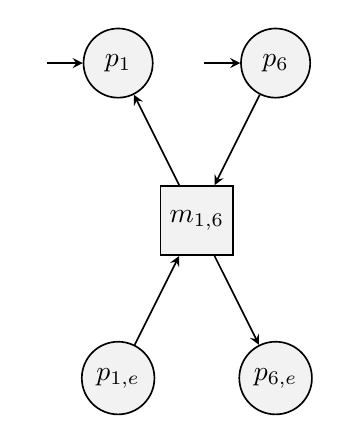
\begin{tikzpicture}
  \node[state, initial] at (3, 4) (p1){$p_1$};
  \node[state, initial] at (5, 4) (p6){$p_6$};

  \node[state] at (3, 0) (p1_e){$p_{1,e}$};
  \node[state] at (5, 0) (p6_e){$p_{6,e}$};

  \node[state, rectangle] at (4, 2) (m1_6){$m_{1,6}$};

  \draw

  (p1_e) edge (m1_6)
  (m1_6) edge (p1)
  (p6) edge (m1_6)
  (m1_6) edge (p6_e)

  ;
\end{tikzpicture}

The Petri Net for $m_{1,11}$

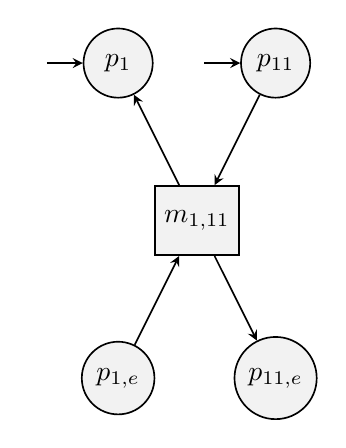
\begin{tikzpicture}
  \node[state, initial] at (3, 4) (p1){$p_1$};
  \node[state, initial] at (5, 4) (p11){$p_{11}$};

  \node[state] at (3, 0) (p1_e){$p_{1,e}$};
  \node[state] at (5, 0) (p11_e){$p_{11,e}$};

  \node[state, rectangle] at (4, 2) (m1_11){$m_{1,11}$};

  \draw

  (p1_e) edge (m1_11)
  (m1_11) edge (p1)
  (p11) edge (m1_11)
  (m1_11) edge (p11_e)

  ;
\end{tikzpicture}

The Petri Net for $m_{2,3}$

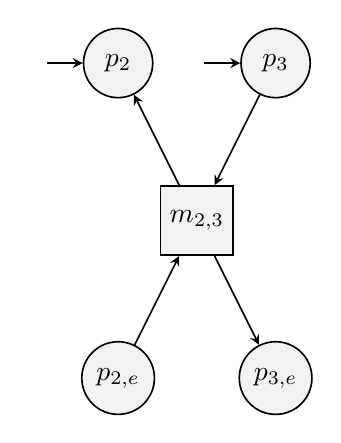
\begin{tikzpicture}
  \node[state, initial] at (5, 4) (p2){$p_2$};
  \node[state, initial] at (7, 4) (p3){$p_3$};

  \node[state] at (5, 0) (p2_e){$p_{2,e}$};
  \node[state] at (7, 0) (p3_e){$p_{3,e}$};

  \node[state, rectangle] at (6, 2) (m2_3){$m_{2,3}$};

  \draw

  (p2_e) edge (m2_3)
  (m2_3) edge (p2)
  (p3) edge (m2_3)
  (m2_3) edge (p3_e)

  ;
\end{tikzpicture}

The Petri Net for $m_{6,3}$

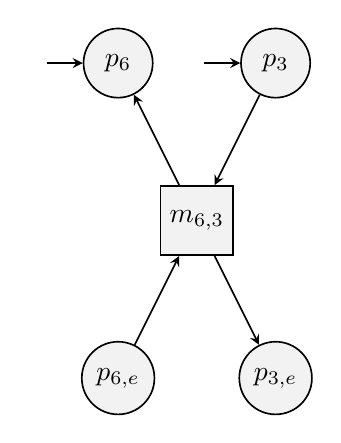
\begin{tikzpicture}
  \node[state, initial] at (5, 4) (p6){$p_6$};
  \node[state, initial] at (7, 4) (p3){$p_3$};

  \node[state] at (5, 0) (p6_e){$p_{6,e}$};
  \node[state] at (7, 0) (p3_e){$p_{3,e}$};

  \node[state, rectangle] at (6, 2) (m6_3){$m_{6,3}$};

  \draw

  (p6_e) edge (m6_3)
  (m6_3) edge (p6)
  (p3) edge (m6_3)
  (m6_3) edge (p3_e)

  ;
\end{tikzpicture}

The Petri Net for $m_{11,3}$

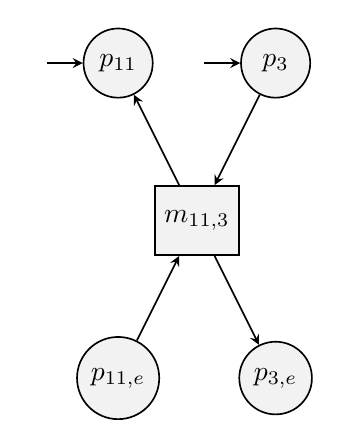
\begin{tikzpicture}
  \node[state, initial] at (5, 4) (p11){$p_{11}$};
  \node[state, initial] at (7, 4) (p3){$p_3$};

  \node[state] at (5, 0) (p11_e){$p_{11,e}$};
  \node[state] at (7, 0) (p3_e){$p_{3,e}$};

  \node[state, rectangle] at (6, 2) (m11_3){$m_{11,3}$};

  \draw

  (p11_e) edge (m11_3)
  (m11_3) edge (p11)
  (p3) edge (m11_3)
  (m11_3) edge (p3_e)

  ;
\end{tikzpicture}

The Petri Net for $m_{5,6}$

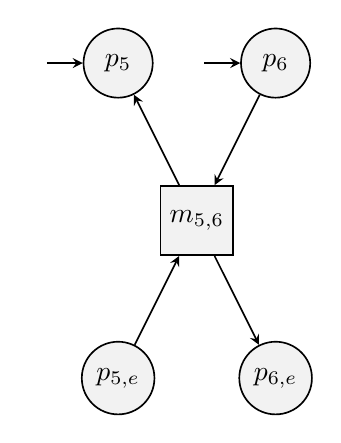
\begin{tikzpicture}
  \node[state, initial] at (3, 4) (p5){$p_5$};
  \node[state, initial] at (5, 4) (p6){$p_6$};

  \node[state] at (3, 0) (p5_e){$p_{5,e}$};
  \node[state] at (5, 0) (p6_e){$p_{6,e}$};

  \node[state, rectangle] at (4, 2) (m5_6){$m_{5,6}$};

  \draw

  (p5_e) edge (m5_6)
  (m5_6) edge (p5)
  (p6) edge (m5_6)
  (m5_6) edge (p6_e)

  ;
\end{tikzpicture}

The Petri Net for $m_{5,11}$

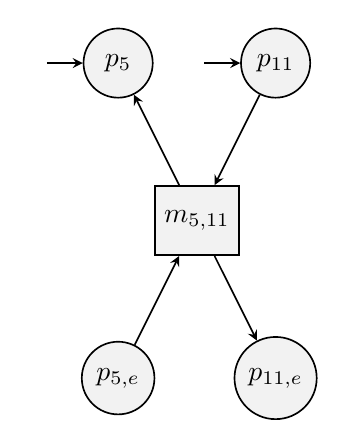
\begin{tikzpicture}
  \node[state, initial] at (3, 4) (p5){$p_5$};
  \node[state, initial] at (5, 4) (p11){$p_{11}$};

  \node[state] at (3, 0) (p5_e){$p_{5,e}$};
  \node[state] at (5, 0) (p11_e){$p_{11,e}$};

  \node[state, rectangle] at (4, 2) (m5_11){$m_{5,11}$};

  \draw

  (p5_e) edge (m5_11)
  (m5_11) edge (p5)
  (p11) edge (m5_11)
  (m5_11) edge (p11_e)

  ;
\end{tikzpicture}

The Petri Net for $m_{10,11}$

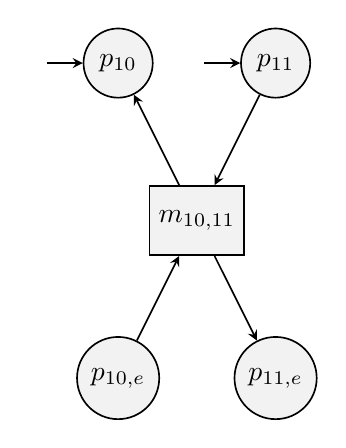
\begin{tikzpicture}
  \node[state, initial] at (3, 4) (p10){$p_{10}$};
  \node[state, initial] at (5, 4) (p11){$p_{11}$};

  \node[state] at (3, 0) (p10_e){$p_{10,e}$};
  \node[state] at (5, 0) (p11_e){$p_{11,e}$};

  \node[state, rectangle] at (4, 2) (m10_11){$m_{10,11}$};

  \draw

  (p10_e) edge (m10_11)
  (m10_11) edge (p10)
  (p11) edge (m10_11)
  (m10_11) edge (p11_e)

  ;
\end{tikzpicture}

\subsubsection{Tracks with Simple Transition (West Direction)}

The Petri Net for $m_{8,7}$

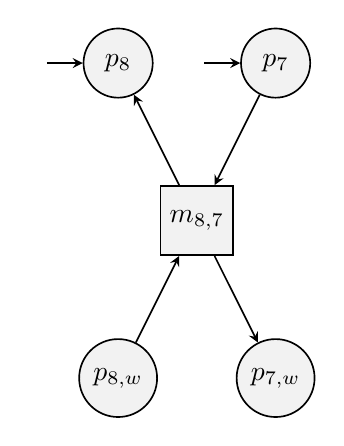
\begin{tikzpicture}
  \node[state, initial] at (5, 4) (p8){$p_8$};
  \node[state, initial] at (7, 4) (p7){$p_7$};

  \node[state] at (5, 0) (p8_w){$p_{8,w}$};
  \node[state] at (7, 0) (p7_w){$p_{7,w}$};

  \node[state, rectangle] at (6, 2) (m8_7){$m_{8,7}$};

  \draw

  (p8_w) edge (m8_7)
  (m8_7) edge (p8)
  (p7) edge (m8_7)
  (m8_7) edge (p7_w)

  ;
\end{tikzpicture}

The Petri Net for $m_{8,12}$

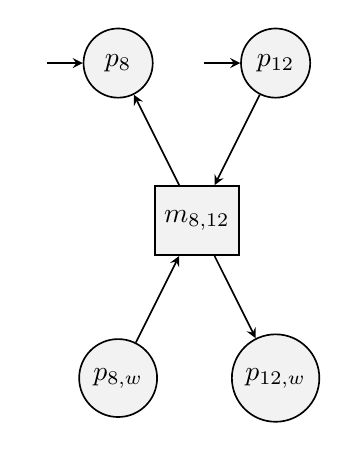
\begin{tikzpicture}
  \node[state, initial] at (5, 4) (p8){$p_8$};
  \node[state, initial] at (7, 4) (p12){$p_{12}$};

  \node[state] at (5, 0) (p8_w){$p_{8,w}$};
  \node[state] at (7, 0) (p12_w){$p_{12,w}$};

  \node[state, rectangle] at (6, 2) (m8_12){$m_{8,12}$};

  \draw

  (p8_w) edge (m8_12)
  (m8_12) edge (p8)
  (p12) edge (m8_12)
  (m8_12) edge (p12_w)

  ;
\end{tikzpicture}

The Petri Net for $m_{12,13}$

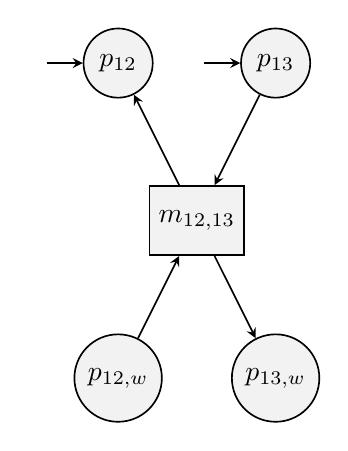
\begin{tikzpicture}
  \node[state, initial] at (5, 4) (p12){$p_{12}$};
  \node[state, initial] at (7, 4) (p13){$p_{13}$};

  \node[state] at (5, 0) (p12_w){$p_{12,w}$};
  \node[state] at (7, 0) (p13_w){$p_{13,w}$};

  \node[state, rectangle] at (6, 2) (m12_13){$m_{12,13}$};

  \draw

  (p12_w) edge (m12_13)
  (m12_13) edge (p12)
  (p13) edge (m12_13)
  (m12_13) edge (p13_w)

  ;
\end{tikzpicture}

The Petri Net for $m_{13,10}$

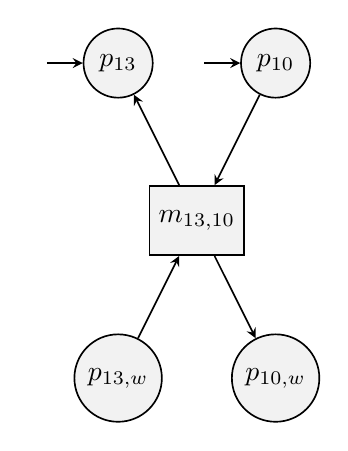
\begin{tikzpicture}
  \node[state, initial] at (5, 4) (p13){$p_{13}$};
  \node[state, initial] at (7, 4) (p10){$p_{10}$};

  \node[state] at (5, 0) (p13_w){$p_{13,w}$};
  \node[state] at (7, 0) (p10_w){$p_{10,w}$};

  \node[state, rectangle] at (6, 2) (m13_10){$m_{13,10}$};

  \draw

  (p13_w) edge (m13_10)
  (m13_10) edge (p13)
  (p10) edge (m13_10)
  (m13_10) edge (p10_w)

  ;
\end{tikzpicture}

The Petri Net for $m_{6,5}$

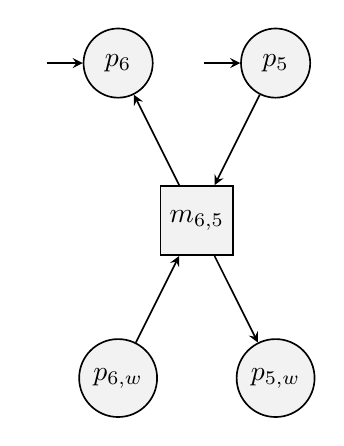
\begin{tikzpicture}
  \node[state, initial] at (5, 4) (p6){$p_6$};
  \node[state, initial] at (7, 4) (p5){$p_5$};

  \node[state] at (5, 0) (p6_w){$p_{6,w}$};
  \node[state] at (7, 0) (p5_w){$p_{5,w}$};

  \node[state, rectangle] at (6, 2) (m6_5){$m_{6,5}$};

  \draw

  (p6_w) edge (m6_5)
  (m6_5) edge (p6)
  (p5) edge (m6_5)
  (m6_5) edge (p5_w)

  ;
\end{tikzpicture}

The Petri Net for $m_{11,5}$

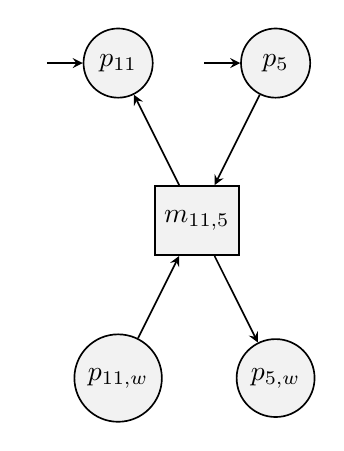
\begin{tikzpicture}
  \node[state, initial] at (5, 4) (p11){$p_{11}$};
  \node[state, initial] at (7, 4) (p5){$p_5$};

  \node[state] at (5, 0) (p11_w){$p_{11,w}$};
  \node[state] at (7, 0) (p5_w){$p_{5,w}$};

  \node[state, rectangle] at (6, 2) (m11_5){$m_{11,5}$};

  \draw

  (p11_w) edge (m11_5)
  (m11_5) edge (p11)
  (p5) edge (m11_5)
  (m11_5) edge (p5_w)

  ;
\end{tikzpicture}

The Petri Net for $m_{11,10}$

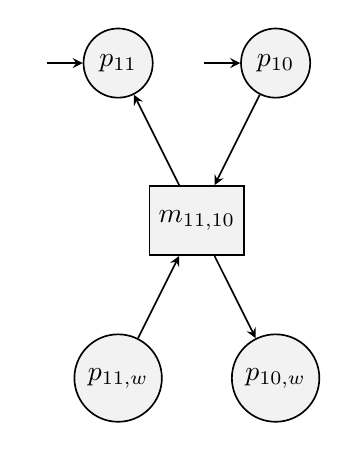
\begin{tikzpicture}
  \node[state, initial] at (5, 4) (p11){$p_{11}$};
  \node[state, initial] at (7, 4) (p10){$p_{10}$};

  \node[state] at (5, 0) (p11_w){$p_{11,w}$};
  \node[state] at (7, 0) (p10_w){$p_{10,w}$};

  \node[state, rectangle] at (6, 2) (m11_10){$m_{11,10}$};

  \draw

  (p11_w) edge (m11_10)
  (m11_10) edge (p11)
  (p10) edge (m11_10)
  (m11_10) edge (p10_w)

  ;
\end{tikzpicture}

The Petri Net for $m_{5,9}$

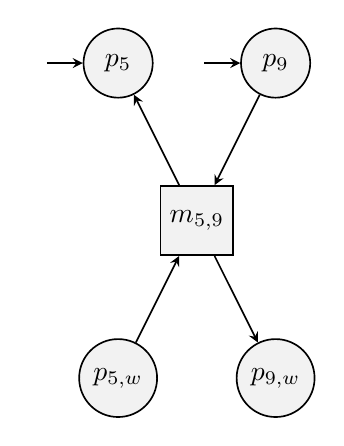
\begin{tikzpicture}
  \node[state, initial] at (5, 4) (p5){$p_5$};
  \node[state, initial] at (7, 4) (p9){$p_9$};

  \node[state] at (5, 0) (p5_w){$p_{5,w}$};
  \node[state] at (7, 0) (p9_w){$p_{9,w}$};

  \node[state, rectangle] at (6, 2) (m5_9){$m_{5,9}$};

  \draw

  (p5_w) edge (m5_9)
  (m5_9) edge (p5)
  (p9) edge (m5_9)
  (m5_9) edge (p9_w)

  ;
\end{tikzpicture}

The Petri Net for $m_{10,9}$

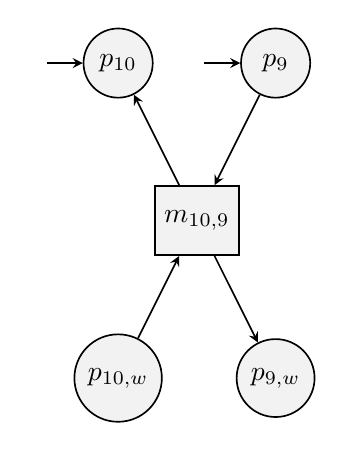
\begin{tikzpicture}
  \node[state, initial] at (5, 4) (p10){$p_{10}$};
  \node[state, initial] at (7, 4) (p9){$p_9$};

  \node[state] at (5, 0) (p10_w){$p_{10,w}$};
  \node[state] at (7, 0) (p9_w){$p_{9,w}$};

  \node[state, rectangle] at (6, 2) (m10_9){$m_{10,9}$};

  \draw

  (p10_w) edge (m10_9)
  (m10_9) edge (p10)
  (p9) edge (m10_9)
  (m10_9) edge (p9_w)

  ;
\end{tikzpicture}

\subsection{Transitions with Potential Deadlock}

Deadlock can happen, as an implication from the simple transitions above, when the current marking contains $$\left\{p_{5,e} \rightarrow 1; p_{10,e} \rightarrow 1; p_{6,w} \rightarrow 1; p_{11,w} \rightarrow 1; \right\}$$. It is important to prevent such a circumstance occurs. That's why I introduce the transition notation as described previously.

\subsubsection{From Track $4$}

When a train wants to entre track $5$ from track $4$, it is necessary to ensure that the current marking should not contain $$\left\{p_{10,e} \rightarrow 1; p_{6,w} \rightarrow 1; p_{11,w} \rightarrow 1; \right\}$$. The simple condition is the same as all other transitions, which is $$\left\{p_5 \rightarrow 1\right\}$$. To ensure the previous mapping will not occur, it is necessary to have either of these extra preconditions before the transition $m_{4,5}$:

\begin{itemize}
  \item $\left\{p_6 \rightarrow 1\right\}$
  \item $\left\{p_10 \rightarrow 1\right\}$
  \item $\left\{p_11 \rightarrow 1\right\}$
  \item $\left\{p_{6,e} \rightarrow 1\right\}$
  \item $\left\{p_{10,w} \rightarrow 1\right\}$
  \item $\left\{p_{11,e} \rightarrow 1\right\}$
\end{itemize}

Each of these can be converted to a part of the Petri Net

\begin{itemize}
  \item
    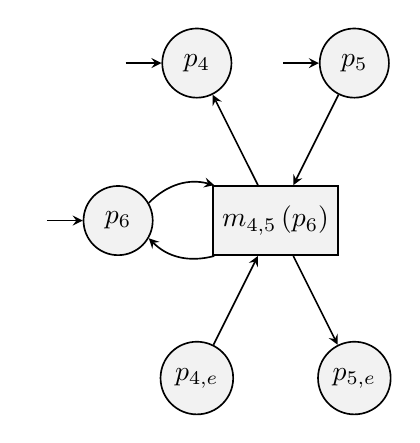
\begin{tikzpicture}
      \node[state, initial] at (1, 4) (p4){$p_4$};
      \node[state, initial] at (3, 4) (p5){$p_5$};
      \node[state, initial] at (0, 2) (p6){$p_6$};

      \node[state] at (1, 0) (p4_e){$p_{4,e}$};
      \node[state] at (3, 0) (p5_e){$p_{5,e}$};

      \node[state, rectangle] at (2, 2) (m4_5){$m_{4,5}\left(p_6\right)$};

      \draw

      (p4_e) edge (m4_5)
      (m4_5) edge (p4)
      (p5) edge (m4_5)
      (m4_5) edge (p5_e)

      (p6) edge[bend left] (m4_5)
      (m4_5) edge[bend left] (p6)

      ;
    \end{tikzpicture}
  \item
    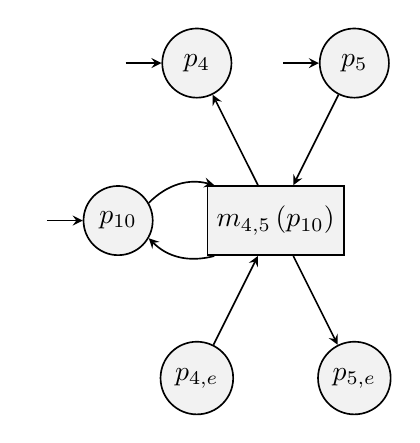
\begin{tikzpicture}
      \node[state, initial] at (1, 4) (p4){$p_4$};
      \node[state, initial] at (3, 4) (p5){$p_5$};
      \node[state, initial] at (0, 2) (p10){$p_{10}$};

      \node[state] at (1, 0) (p4_e){$p_{4,e}$};
      \node[state] at (3, 0) (p5_e){$p_{5,e}$};

      \node[state, rectangle] at (2, 2) (m4_5){$m_{4,5}\left(p_{10}\right)$};

      \draw

      (p4_e) edge (m4_5)
      (m4_5) edge (p4)
      (p5) edge (m4_5)
      (m4_5) edge (p5_e)

      (p10) edge[bend left] (m4_5)
      (m4_5) edge[bend left] (p10)

      ;
    \end{tikzpicture}
  \item
    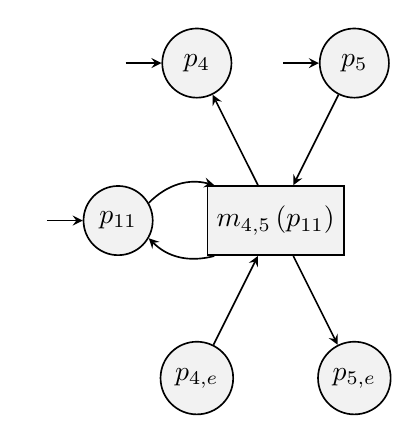
\begin{tikzpicture}
      \node[state, initial] at (1, 4) (p4){$p_4$};
      \node[state, initial] at (3, 4) (p5){$p_5$};
      \node[state, initial] at (0, 2) (p11){$p_{11}$};

      \node[state] at (1, 0) (p4_e){$p_{4,e}$};
      \node[state] at (3, 0) (p5_e){$p_{5,e}$};

      \node[state, rectangle] at (2, 2) (m4_5){$m_{4,5}\left(p_{11}\right)$};

      \draw

      (p4_e) edge (m4_5)
      (m4_5) edge (p4)
      (p5) edge (m4_5)
      (m4_5) edge (p5_e)

      (p11) edge[bend left] (m4_5)
      (m4_5) edge[bend left] (p11)

      ;
    \end{tikzpicture}
  \item
    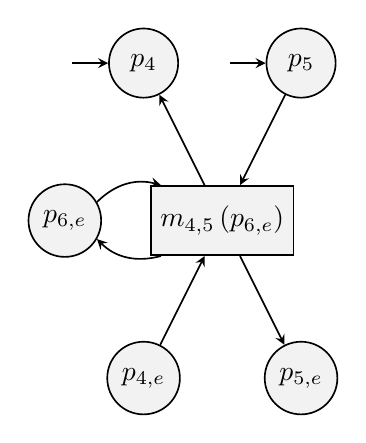
\begin{tikzpicture}
      \node[state, initial] at (1, 4) (p4){$p_4$};
      \node[state, initial] at (3, 4) (p5){$p_5$};
      \node[state] at (0, 2) (p6_e){$p_{6,e}$};

      \node[state] at (1, 0) (p4_e){$p_{4,e}$};
      \node[state] at (3, 0) (p5_e){$p_{5,e}$};

      \node[state, rectangle] at (2, 2) (m4_5){$m_{4,5}\left(p_{6,e}\right)$};

      \draw

      (p4_e) edge (m4_5)
      (m4_5) edge (p4)
      (p5) edge (m4_5)
      (m4_5) edge (p5_e)

      (p6_e) edge[bend left] (m4_5)
      (m4_5) edge[bend left] (p6_e)

      ;
    \end{tikzpicture}
  \item
    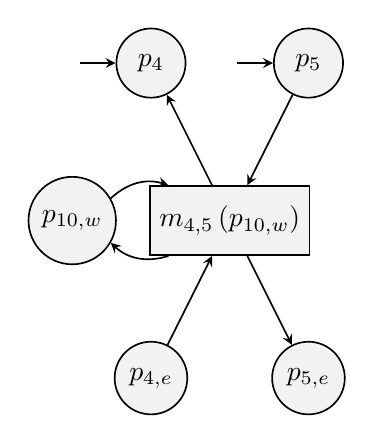
\begin{tikzpicture}
      \node[state, initial] at (1, 4) (p4){$p_4$};
      \node[state, initial] at (3, 4) (p5){$p_5$};
      \node[state] at (0, 2) (p10_w){$p_{10,w}$};

      \node[state] at (1, 0) (p4_e){$p_{4,e}$};
      \node[state] at (3, 0) (p5_e){$p_{5,e}$};

      \node[state, rectangle] at (2, 2) (m4_5){$m_{4,5}\left(p_{10,w}\right)$};

      \draw

      (p4_e) edge (m4_5)
      (m4_5) edge (p4)
      (p5) edge (m4_5)
      (m4_5) edge (p5_e)

      (p10_w) edge[bend left] (m4_5)
      (m4_5) edge[bend left] (p10_w)

      ;
    \end{tikzpicture}
  \item
    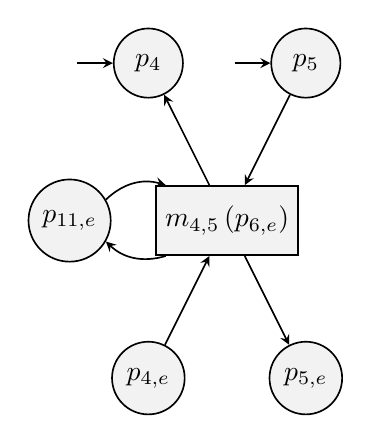
\begin{tikzpicture}
      \node[state, initial] at (1, 4) (p4){$p_4$};
      \node[state, initial] at (3, 4) (p5){$p_5$};
      \node[state] at (0, 2) (p11_e){$p_{11,e}$};

      \node[state] at (1, 0) (p4_e){$p_{4,e}$};
      \node[state] at (3, 0) (p5_e){$p_{5,e}$};

      \node[state, rectangle] at (2, 2) (m4_5){$m_{4,5}\left(p_{6,e}\right)$};

      \draw

      (p4_e) edge (m4_5)
      (m4_5) edge (p4)
      (p5) edge (m4_5)
      (m4_5) edge (p5_e)

      (p11_e) edge[bend left] (m4_5)
      (m4_5) edge[bend left] (p11_e)

      ;
    \end{tikzpicture}
\end{itemize}

The rest of the transitions will follow the same principles, and I think it will be a bit superfluous to draw all of these. Those transitions are

\begin{itemize}
  \item $m_{4,10}$
  \item $m_{7,6}$
  \item $m_{7,11}$
  \item $m_{12,11}$
\end{itemize}

And everything discussed above will form the final Petri Net.

\section{Priority}

Although Petri Net is non-deterministic, but the selection of transition can affect the overall efficiency of the system. For example, when track $2$, $6$ and $11$ are empty, a train coming from $1$ should prioritise the transition to track $2$ but neither $6$ or $11$. It is quite obvious that $2$ will only be accessible from $1$, thus it will not block any other train lines. The similar reason can be applied to track $12$ as $13$ must be chosen as the first priority in the transition list. As listed in the previous section that $m_{12,11}$ is will potentially incur a deadlock, this is the first step to avoid deadlock happens.

\end{document}
